\chapter{PROPOSED SOLUTION}
\label{chap:solution}
\section{Data collecting with crowd-sourcing model}
A traditional method of collecting data is to do it manually : Setting up an array of cameras at desired locations and then obtain their recordings. Those recording would later be labeled by specialists or experts and processed to form a dataset. This way of approach is expensive and requires a lot of human resources.

One other method of data collection is to implement Web crawler to pull data from the internet automatically. This method would be most useful for getting a large amount of data given a keyword. One downside is that data achieved by this method often contain considerable noise because of typos, mislabel or error. In the context of security, those data are not suitable to be used because they are incredibly diverse and do not portray the Vietnamese environment accurately. Moreover, public data used for security matter can be collected by crawler is not considerable or may insufficient.

Crowd-sourcing is also one of the effective methods of data collection which is becoming a trend in the last couple of years. The idea behind crowd-sourcing data is to build datasets with the assistance of the community. An example of this kind of model is Wikipedia\footnotetext{\url:{https://www.wikipedia.org}}
. Wikipedia is an enormous web-based, collaborative encyclopedia which has over 100,000 volunteers contributing new information to the system daily. The success of Wikipedia proves the capability of crowd-sourcing. The solution is applicable to this project due to its advantages of significant cost saving. Furthermore, appropriate datasets can be created by Vietnamese community.

However, how can people be encouraged to provide their knowledge and information? Interaction with others is proven successful in encouraging people to share.Therefore, social media has been a popular trend among Vietnamese in recent years. At the time of November 2018, the amount of people using Facebook has reached about 70 million, that accounts for almost 73\% of the population. (Figure \ref{chap3:social_media_vn}).

Because of mentioned factors, this thesis proposes building a \textbf{Social media website for security} where users can interact with each other, as well as provide their data to the system via posting.
\begin{center}
    \begin{figure}[H]
    \centering
    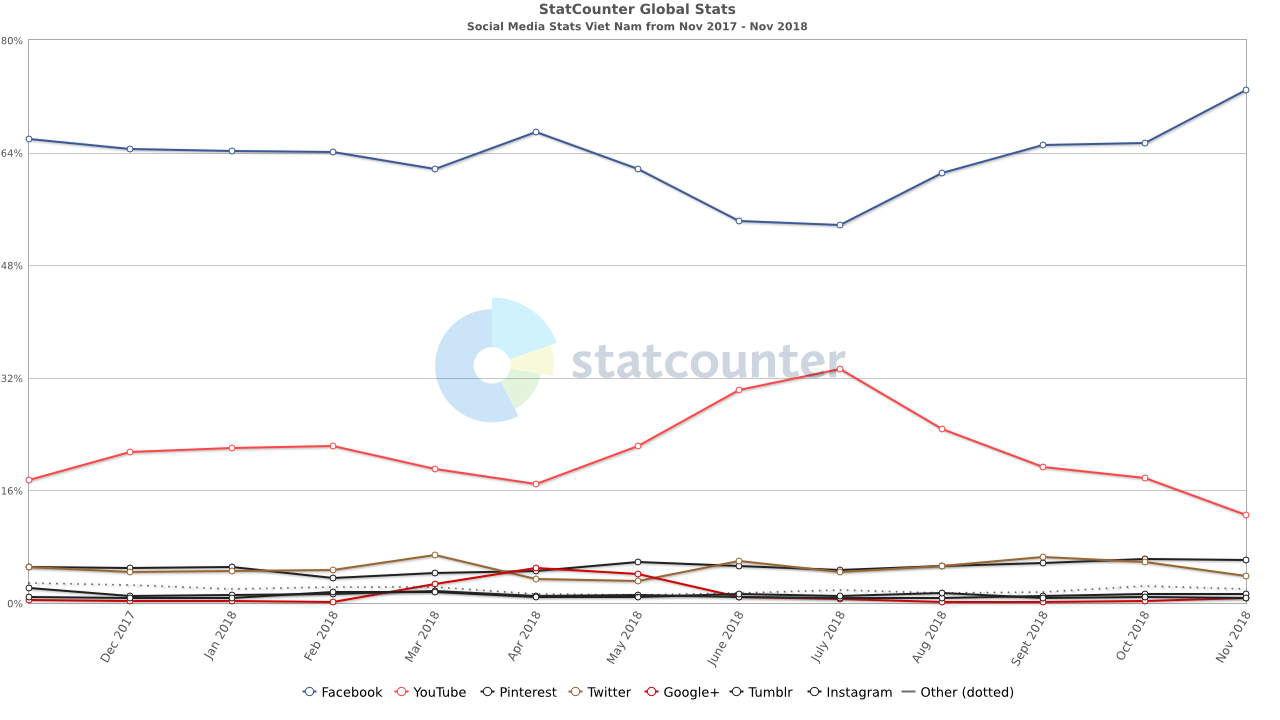
\includegraphics[width=1\columnwidth]{images/chap3/social_media_vn.png}
    \footcaption{Social media usage of Vietnamese is at all time high. Nearly 73\% of the population is using use Facebook}
    \label{chap3:social_media_vn}
    \end{figure}
\end{center}
\footnotetext{Source: \url:{http://gs.statcounter.com/social-media-stats/all/viet-nam}}
\section{Extracting information from data}
\subsection{Image}
\subsection{Video}

